\documentclass{article}
\usepackage{graphicx}
\usepackage[margin=1.5cm]{geometry}
\usepackage{amsmath}

\begin{document}
\twocolumn

\title{Lab Activity: Center of Mass, Torque, and Static Equilibrium}
\author{Prof. Jordan C. Hanson}

\maketitle

\section{Introduction}

\noindent
In this lab, we are investigating \textit{static equilibrium}.  A system experiences static equilibrium if the following two conditions are met: (1) The net external force is zero, and (2) the net external torque is zero.  In the form of equations, conditions (1) and (2) are

\begin{align}
\sum_i \vec{F}_i &= 0 \\
\sum_i \vec{\tau}_i &= 0
\end{align}

\noindent
Consider \ref{fig:1}.  The pivot $S$ provides enough normal force to support the weight of $m_1$, $m_2$, $m_3$, and the ruler with mass $m_r$.  Thus, the net force is zero and condition (1) is met.  To find the net torque, note that $m_1 = 50$ grams, $m_2 = 75$ grams, and $m_r = 150$ grams.  We would like to find an $m_3$ that achieves balance, but how do we calculate the torque due to $m_r$?

\section{The Center of Mass}

\noindent
A \textit{weighted average} for a set of data points $x_i$ and \textit{weights} $w_i$ is calculated as follows:

\begin{align}
1 &= \sum_i w_i \\
\bar{x} &= \sum_i w_i x_i
\end{align}

\noindent
That is, we ensure the weights sum to 1, and then multiply each data point by a weight, to give it more or less weight in the average.  If all the weights are equal, then the weighted average reverts to the arithmetic mean, or regular average.  Suppose we want to compute the weighted average location of the ruler, weighted by mass:

\begin{align}
M &= \sum_i m_i \\
\vec{r}_{\rm CM} &= M^{-1} \sum_i m_i \vec{r}_i
\end{align}

\noindent
This vector is known as the \textit{center of mass.}  Show that, if we chop the ruler into 100 equal pieces, $\vec{r}_{\rm CM}$ is located approximately where the ruler reads 50 cm. \\ \vspace{3cm}

\section{The Net Torque}

\noindent
Now that we know where the center of mass is located, calculate the torque due to $m_r$ by letting the $\vec{r}$ in $\vec{r} \times \vec{F}$ be $\vec{r}_{\rm CM}$: \\ \vspace{3cm}

\noindent
Solve for $m_3$ such that the net torque is zero: \\ \vspace{3cm}

\section{Lab Measurement}

\noindent
Recreate the situation in Fig. \ref{fig:1} using the rulers, pivot weights, and masses provided.  Record below the locations of the masses, and calculate the net torque.  Does the system balance?

\begin{figure}
\centering
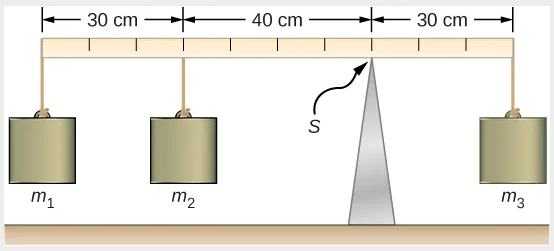
\includegraphics[width=0.4\textwidth]{figures/balance.png}
\caption{\label{fig:1} A torque balance.}
\end{figure}

\end{document}
